\chapter{Evaluating Dimensionality Reduction Methods for Genomic Prediction}
    
\section{Introduction}

Plant breeding techniques have lead to significant gains in crop yields for many decades. Improvements to crops were made through phenotypic and pedigree data. The use of molecular markers is a relatively new technique for improving conventional breeding strategies. Most traits that have economic and agronomic importance are quantitative in nature and are controlled by multiple genes of small effect. The advent of high-throughput genotyping and Single Nucleotide Polymorphisms (SNPs) led to methods such as Marker-assisted Selection (MAS) where favorable individuals could be selected using a limited number of previously identified markers that were highly associated with the trait of interest. The drawbacks of MAS include complexity in identifying associated QTLs across environments and difficulty in improving the prediction of complex traits due to their dependence on multiple genes.\\

The ever-reducing cost of SNP assays brought forward the possibility of using dense SNP arrays for the prediction of phenotypic traits. Genomic selection (GS) proposed by \cite{meuwissen_prediction_2001} is an extension of MAS, where the entire genome is used to predict the phenotypic traits instead of using a selected subset of markers as in MAS. Phenotypic and genotypic data from the training set are used to estimate the breeding values (known as genomic estimated breeding values - GEBVs) of the testing set. The testing set contains the genomic information of the lines but not their phenotypic information. Since GS does not depend on phenotypic data of the testing set, it allows for faster development of the breeding program. Phenotypic data collection is often the more expensive component in a breeding program and hence GS also helps cut costs. \cite{bernardo_prospects_2007} presented the genetic gains of GS compared to MAS using simulated data. It has been shown that GS has better prediction accuracy than pedigree-based prediction models as genetic marker data take into consideration the segregation effects \cite{de_los_campos_predicting_2009, crossa_genomic_2011, crossa_prediction_2010}. \\

A major challenge of GS lies in estimating the large number of marker effects ($p$) using information from only a few number of individuals $n$. Many models and algorithms have been proposed in literature to overcome this challenge. Some of the prominent shrinkage-based models include ridge-regression BLUP, BayesA and BayesB \cite{meuwissen_prediction_2001}, LASSO \cite{usai_lasso_2009}, elastic net \cite{zou_regularization_2005}, Bayesian LASSO \cite{de_los_campos_predicting_2009}, reproducing kernel Hilbert spaces \cite{gianola_genomic-assisted_2006, de_los_campos_semi-parametric_2010}, and support vector regression \cite{moser_comparison_2009, long_application_2011}. While these models deal with the dimensionality issue through shrinkage methods, they did not incorporate multi-environment information.\\

Environment and genotype by environment (G $\times$ E) interactions strongly impact the performance of lines from one environment to the next and hence accounting for these effects could improve the performance of the prediction models \cite{roorkiwal_genomic-enabled_2018, jarquin_increasing_2017}.  \cite{burgueno_genomic_2012} included the genotype by environment (G $\times$ E) information through structured genetic correlations and found that using multi-environment information improved the prediction accuracy. \cite{jarquin_reaction_2014} proposed the multiplicative reaction-norm model (MRNM), an extension to the standard G-BLUP model and an alternative to the models proposed by \cite{burgueno_genomic_2012}. The MRNM models allowed for the environmental effect to be included along with the genomic information and the G $\times$ E interaction effect by modeling the covariance structure. They showed that introducing interactions between the environmental covariates and molecular markers can increase the proportion of variance explained by the model as well as increase the prediction accuracy. \\

Most of these methods deal with the high-dimensional aspect of genomic selection through modern shrinkage procedures. Shrinkage methods perform dimensionality reduction as a part of the modeling process. In this paper, we examine the utility of dimensionality reduction (DR) methods as a pre-processing step to genomic prediction. In ``small $n$ large $p$" problems such as genomic prediction, several markers (aka variables or features) may be insignificant in explaining the phenotypic response. Thus, it is essential to eliminate such insignificant features to improve the prediction process. Eliminating irrelevant features before running prediction models could also help in reducing the resource requirements for the computations of the models in terms of memory as well as time. \\

The primary objective of this work is to study the  utility of implementing dimensionality reduction as a pre-processing step in genomic prediction. We employed five different DR methods and investigated their ability to improve genomic prediction. Further, we compared their relative reduction abilities to potentially identify methods that worked better than others. We were also interested in studying the trend in the prediction accuracy as a function of the number of markers retained from the original marker data. Another objective of the study was to evaluate the DR methods on a real data set. In order to answer these objectives, we created 26 reduced data sets with sequentially increasing number of markers using each of the DR methods, performed genomic prediction for each size, and computed their respective prediction accuracy values. Our hypothesis was that the prediction accuracy values would plateau beyond a certain size and any further increase in the number of markers in the input data set would not significantly improve and potentially even harm the prediction accuracy. \\

The rest of the paper is organized as follows. First, we present the different DR methods in the Material and Methods section. Here, we review some key definitions and notations that will be used in the rest of the paper and present a detailed overview of each of the five reduction methods. For each method, we also describe their implementation in the context of creating reduced marker data sets. Next, we describe the genomic prediction concept by detailing the statistical models and cross-validation schemes used, along with a description of the real data set. Following that, we present the results of the DR for each method along with comparisons. Finally, we conclude with discussion and future directions.  \\

\section{Materials and Methods}
\subsection{Dimensionality Reduction}

Traditional methods and approaches to data analysis are proving to be unsuitable in the face of massive modern data sets. The need of the hour dictates development of new statistical algorithms that are able to analyze these large data sets. The objective of these new algorithms is to work within reasonable constraints on computational resources and time while providing reliable solutions to research problems. With ever-increasing access to storage resources and reduction in the cost of collecting additional features on observational units, the dimension of data sets is constantly increasing. For instance, the advent of high-throughput phenotyping and genotyping technologies in life-sciences has lead to the generation of huge data sets which present unprecedented storage and computational challenges. \\

High-dimensional data could be classified as `large $n$, large $d$' datasets or `small $n$, large $d$' datasets. A primary assumption in the analysis of such high-dimensional data is the existence of a lower-dimensional subspace which contains all of the important information and allows for reliable inference as well as prediction of the response variable. Given a matrix $\boldsymbol{A} \in \boldsymbol{\mathds{R}}^{n \times d}$, obtaining a `compressed' matrix that captures the most important and relevant information present in $\textbf{A}$ has significant practical importance. The process of obtaining this compressed matrix is referred to as dimensionality reduction. Dimensionality reduction assumes greater importance in the case of computations involving high-dimensional data sets. Low rank approximations for such matrices are commonly used in various statistical applications such as principal components analysis (PCA), k-mean clustering, data compression, solving linear equations, etc.   \\

It is well known that the best rank-$k$ approximation of any matrix is obtained by the Singular Value Decomposition (SVD) \cite{eckart_approximation_1936}. Although SVD provides the best rank-k approximation of a matrix, it is increasingly infeasible to compute it due to the sheer size of modern data sets. Consider again the matrix $\boldsymbol{A} \in \boldsymbol{\mathds{R}}^{n \times d}$ and without loss of generality, assume that $d >n$. The computation of the best rank-k approximation $\textbf{A}_k$ takes $O(nd^2)$ time \cite{golub_matrix_2013}, which can prove prohibitive for modern large data sets. Recent decades have witnessed substantial progress in the development of several DR methods to obtain accurate low-rank representations of matrices, while overcoming the computational challenges presented by SVD. These algorithms compute a low-rank approximation that can replace the original matrix in computations without loss in precision.  \\

DR methods can be categorized into three main approaches \cite{ghashami_frequent_2015}: sparsification, feature extraction and feature selection. Sparsification refers to generating a sparse version of the matrix which can be stored efficiently and lead to faster matrix multiplication \cite{achlioptas_fast_2007, drineas_note_2011}. Low rank approximations of a matrix can also be generated by linear combinations of the original features to form new combined features. These linear combinations are determined through pre-multiplication of the original features with a coefficients matrix and this approach is called feature extraction. PCA \cite{pearson1901} and LDA \cite{fisher_use_1936} are two popular algorithms for feature extraction to project the data onto a lower dimensional representation. The third approach -- called feature selection -- refers to a method where we find a small subset of the original features that approximate the whole set of features. Forward selection, backward selection, and best subset selection \cite{james_introduction_2013} algorithms are commonly used feature selection algorithms. Feature selection is equivalent to the column subset selection problem (CSSP) in numerical linear algebra, which has been well studied and has seen several applications in data analysis \cite{boutsidis_improved_2009, deshpande_matrix_2006, drineas_fast_2012, drineas_fast_2006, drineas_sampling_2006, drineas_relative-error_2008, drineas_faster_2011, mahoney_cur_2009, papailiopoulos_provable_2014}. \\

The feature extraction method yields a compressed matrix that is formed by computing linear combinations of the original features. While this method has been shown to provide reliable approximations to the original data matrix for further computations, there is an obvious issue in working with combination of features. The linear combinations may not be suitable to make statistical inferences about the original data scale and there may be no sensible interpretation of the combinations themselves in certain applications. Given this drawback of the feature extraction method, the feature selection approach to dimensionality reduction presents itself as a more suitable choice. The feature selection method involves selecting a small subset of the original features to create a compressed features matrix and hence avoids the issues related to inference and interpretability. For this reason, we examined the feature selection approach in greater detail by investigating four feature selection based algorithms. Each of these methods presents a fundamentally different approach to feature selection. \\

DR methods can also be categorized as deterministic or randomized methods based on the way in which the lower dimensional representation is derived. In deterministic methods, features are selected in a fixed manner based on some property of the data such as the singular values as in the case of PCA. Features are also often selected based on model fit statistics such as Akaike information criterion (AIC) and Bayesian information criterion (BIC) as in the case of forward selection. Randomized algorithms were proposed as an alternative approach that reduce the computational resource requirement and provide faster solutions than deterministic methods \cite{drineas_relative-error_2008, clarkson_low-rank_2017, ailon_fast_2009, achlioptas_fast_2007, sarlos_improved_2006, liberty_randomized_2007, frieze_fast_2004, tropp_practical_2017}. These methods provide approximations to the exact solutions in less time by trading accuracy for efficiency in solving high-dimensional problems \cite{musco_power_2018}. In randomized algorithms, features are selected or extracted at random based on some probability distribution. Choosing a well-suited probability distribution ensures that the approximations are of high quality. \\

In this paper, we focused only on the feature selection and feature extraction approaches to dimensionality reduction. We examined the ability of five methods to reduce the dimensionality of the predictor data set in the context of the genomic prediction problem. Specifically, we compared the random projection algorithm proposed by \cite{ailon_fast_2009} to four feature selection algorithms based on random sampling \cite{boutsidis_improved_2009}, deterministic sampling \cite{papailiopoulos_provable_2014}, ridge regression \cite{hoerl_ridge_1970}, and clustering \cite{sneath_numerical_1973}. Random sampling and random projection methods are often referred together as random sketching methods. Out of these five methods, we applied a randomized approach to three of them - random projection, random sampling, and a clustering based feature selection algorithm. We compared these to two deterministic algorithms based on deterministic sampling and ridge regression. The five methods are summarized in Figure \ref{fig: dimRed_methods}. \\

\begin{center}
\begin{figure}[!t]
\centering
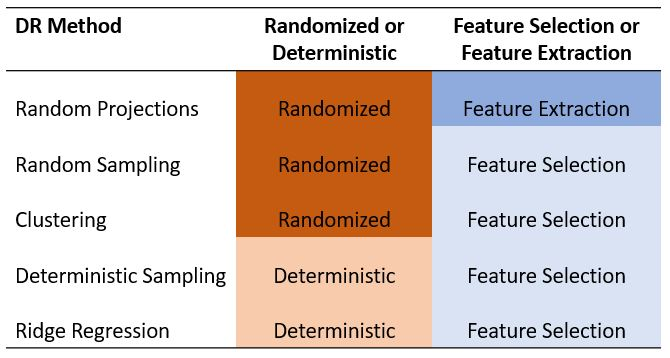
\includegraphics[scale=0.6]{figures/dim_red_methods_chart_2.JPG}
\caption{Summary of the five dimensionality reduction methods used in this paper. The methods are categorized as feature selection/feature extraction and as randomized/deterministic. }
\label{fig: dimRed_methods}
\end{figure}
\end{center}

\subsection{Background}
\label{sec:background}
Before we present the relevant literature for each of the DR methods, we review some key linear algebra definitions and notations. 

\begin{itemize}
\item We use $e_j$ to denote the $j$-th standard basis vector in  $\mathds{R}^n$, i.e., $e_j$ is a vector with its $j$-th entry equal to 1 and all other entries equal to 0.
\item Throughout this paper, $||\cdot||_2$ is  used to denote the spectral norm. We also use $||\cdot||_F$ to denote the Frobenius norm. The spectral and Frobenius norms of a matrix $\textbf{A} \in \mathds{R}^{m\times n}$ are defined as:

\begin{eqnarray*}
||\textbf{A}||_2 &=&  \sup_{x\in \mathds{R}^n, x\neq 0} \frac{|Ax|}{|x|},\ \text{and} \\
||\textbf{A}||_F &=& \sqrt{\sum_{i=1}^m \sum_{j=1}^n a_{ij}^2},
\end{eqnarray*}

where $a_{ij}$ are elements in matrix $\textbf{A}$ and $|\cdot|$ is the Euclidean vector norm defined as $|x| = \sqrt{\sum_{i=1}^n x_i^2}$. 

\end{itemize}

Statistical leverage scores have been an integral part of data analysis for many decades. They are a measure of how well the singular vectors of a matrix are correlated with the standard basis and thus have been used for outlier detection in regression analysis \cite{hoaglin_hat_1978, chatterjee1988}. Statistical leverages scores can also be interpreted as the amounted of leverage or influence a data point has \cite{velleman_efficient_1981}, and hence have found application in randomized matrix algorithms \cite{drineas_fast_2012, drineas_relative-error_2008, mahoney_cur_2009, drineas_faster_2011}. Leverage scores of the columns of a matrix are defined as the squared Euclidean norms of the columns of the matrix containing the top right singular vectors. More formally, \\

\textbf{Definition:} Given a matrix $\textbf{A} \in \mathds{R}^{n\times d}$, let $V'$ denote the matrix containing the top right singular vectors of $\textbf{A}$. Then, the statistical leverage score of the $i$-th column of $\textbf{A}$ is defined as,

\begin{equation}
l_i = \left\Vert V'_{(i)} \right\Vert_2^2 \ \ \forall\ i =1, 2,  \dots, d
\end{equation}

\noindent where $V'_{(i)}$ is the $i$-th column of the matrix $V'$. The computational bottleneck lies in the exact computation of $V'$, requiring $O(n^2d)$ time. This bottleneck can be avoided by calculating the relative-error approximations to the statistical leverage scores \cite{drineas_fast_2012}. \\


\subsection{Random Sketching}
\label{sec:random sketching}
In order to understand the need for a random sketching algorithm, let us consider the simple example of linear regression. Suppose we have a $ \textbf{X} \in \mathds{R}^{n \times d}$ full rank matrix of predictor variables and a response vector $\textbf{y}$ of length $n$. The least squares estimates can be computed as, 

\begin{equation*}
\hat{\beta} =  (\textbf{X}'\textbf{X})^{-1} \textbf{X}'\textbf{y}.
\end{equation*}

Thus, we need the Gram matrix $\textbf{X}'\textbf{X}$ and $\textbf{X}'\textbf{y}$ to compute the solution. The computation of $\textbf{X}'\textbf{X}$ requires $O(nd^2)$ time and $\textbf{X}'\textbf{y}$ requires $O(nd)$ time.  When $n > d$, this solution is easy to calculate and is very popular in practice. But, when $n, d$ or both are large --- as they tend to be in many modern data sets --- this computational time can be practically prohibitive. \\

Random sketching is a popular method to reduce the computational complexity of this problem.  Instead of using the full data set $(\textbf{X}, \textbf{y})$, we can employ a carefully constructed sketch $(\tilde{\textbf{X}},\tilde{\textbf{y}})$ to solve for the least squares coefficients. We define $\tilde{\textbf{X}} = \textbf{S}\textbf{X}$ and $\tilde{\textbf{y}}= \textbf{S}\textbf{y}$, where $\textbf{S}$ is a randomly generated ``sketching matrix" of size $r \times n$, $r << n$. The least squares solution will then be given by, 

\begin{equation*}
\hat{\beta_s} = (\tilde{\textbf{X}}'\tilde{\textbf{X}})^{-1} \tilde{\textbf{X}}'\tilde{\textbf{y}},
\end{equation*}

\noindent where $\hat{\beta_s}$ refers to the sketched solution. The cost of computing this solution reduces to $O(rd^2)$. For a sketched solution, our two primary goals are to ensure that the approximate solution is close to the original and to ensure that the computational time is significantly reduced. The careful construction of the sketching matrix $\textbf{S}$ helps us achieve both these goals. In the next section, we present the Johnson-Lindenstrauss Lemma and its role in random sketching algorithms. Following that, we explore literature to identify different choices for $\textbf{S}$ and their relative advantages and disadvantages.  \\

\subsubsection{Johnson-Lindenstrauss Lemma and its extensions}

Dimensionality reduction involves some form of mapping data from a high-dimensional space to a lower dimensional space in such a manner that the information from the original data is retained. The existence of a mapping that can approximately preserve pairwise distances while embedding data from a high-dimensional space into a lower-dimensional space was guaranteed by a lemma by \cite{JL1984} and is commonly known as the Johnson Lindenstrauss Lemma (JL Lemma). JL Lemma is a fundamental component of all random projection algorithms and hence we present a brief summary of the lemma and its extensions before discussing random projection. \\

\cite{JL1984} showed that $n$ points in an Euclidean space $\mathds{R}^d$ can be projected onto a $r= O(\log n /\epsilon^2)$ dimensional space without distorting any pairwise distances of the $n$ points by more than a factor of $(1\pm\epsilon)$ for any $\epsilon \in (0, 1/2]$. Johnson and Lindenstrauss provided this lemma as a tool to prove extensions of Lipschitz mapping into a Hilbert space. But due to its distance preserving nature, it has become a popular tool in dimensionality reduction. \\

\textbf{JL Lemma:} For any $\epsilon \in (0, 1/2]$ and any set of $n$ points $x_1, x_2, \dots, x_n$ in $\mathds{R}^d$, there exists a projection map $f: \mathds{R}^d \rightarrow \mathds{R}^r$, where $r= O(\log n /\epsilon^2)$. Then, for all $i,\  j \in \{1, 2, \dots, n\}$, 

\begin{equation}
(1-\epsilon)\Vert x_i-x_j \Vert_2^2 \leq \Vert f(x_i)-f(x_j)\Vert_2^2 \leq (1+\epsilon)\Vert x_i-x_j \Vert_2^2.
\end{equation}



Johnson and Lindenstrauss provided a lengthy technical proof using geometric approximation. Their main idea was summarized succinctly by  \cite{fedoruk_dimensionality_2018}:

\begin{itemize}
\item Project a set of points $x_1, x_2, \dots, x_n$ in  $\mathds{R}^d$ onto a random $r$- dimensional space. 
\item The expected length of each $r$-dimensional vector is $\sqrt{r/d}$ times the length of the original vectors. 
\item Multiplying each projection by  scaling factor of $\sqrt{d/r}$ yields $r$-dimensional vectors which are similar in length to the original $d$-dimensional vectors. 
\item If we choose a tolerance limit $\epsilon$, then with non-zero probability each length is preserved within the chosen tolerance limit. 
\end{itemize}

The JL Lemma has had numerous improvements and extensions over time. The improvements were two-pronged: improvements in the bounds for $r$ and improvements to the efficiency of $f(\cdot)$. The original proof by Johnson and Lindenstrauss suggested the lower bound for $r$ as $O(\log n /\epsilon^2)$. \cite{frankl1988} improved the lower bound to $r = O(9\log n /(\epsilon^2 - 2\epsilon^3/3))$. Further, they also provided a method to find a suitable mapping. JL Lemma only proves the existence of a mapping function $f(\cdot)$, but does not provide a way of finding one. \cite{dasgupta_elementary_2003} relied on probabilistic techniques to improve the lower bound results to $r= O(4\log n /(\epsilon^2/2 - 2\epsilon^3/3))$. Their proof is also considered significantly simpler than the original proof by \cite{JL1984}. Both these papers retained the definition of the random projection from the original paper, summarized below \cite{ailon_fast_2009} :

\begin{itemize}
\item Spherical symmetry: For any orthogonal matrix $A$, $A$ and $f(A)$ have the same distribution.
\item Orthogonality: The rows of $f(\cdot)$ are orthogonal to each other.
\item Normality: The rows of $f(\cdot)$ are unit-length vectors.
\end{itemize}

Improvements in the efficiency of $f(\cdot)$ were made through relaxing the assumptions listed above. \cite{har-peled_approximate_2012}  showed that the JL Lemma could be satisfied even without the  orthogonality and normality conditions being met. They proposed a projection matrix $R$ where each element of the matrix was sampled from the $N(0, 1/d)$ distribution. \\

\subsection{Random projection}

Random projection algorithms form one of the major class of random sketching algorithms. Random projection algorithms “uniformize” the non-uniformity structure present, by rotating the matrix to a basis where the uniform random sampling of features is nearly optimal. Random projection can be viewed as the process of dimensionality reduction with the objective of preserving the pairwise distances between observations. \\

Random projection produces matrices that are formed by a small number of linear combinations of all of the original features. The resulting compressed matrix can be used as a substitute in computations, thereby reducing the computational complexity of the problem at hand. The linear combinations are formed through pre-multiplying the features with a randomly generated coefficients matrix, and hence the name `random' projection. Given below is a simple random projection algorithm: 

\begin{itemize}
\item Consider an input matrix $\textbf{A} \in \mathds{R}^{n\times d}$ with $d >> n$ without loss of generality.
\item Construct a $d \times k$ random projection matrix $\textbf{S}$, where $k << n$.
\item Obtain the sketched matrix $\textbf{B}= \textbf{A}\textbf{S}$, where $\textbf{B}$ is a $n \times k$ matrix. 
\end{itemize}

\begin{center}
\begin{figure}[!t]
\centering
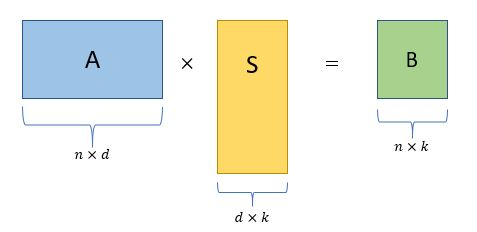
\includegraphics[scale=0.8]{figures/rp_1.JPG}
\caption{Schematic for a simple random projection.}
\label{fig:rp_scheme}
\end{figure}
\end{center}

Let us consider the example of performing the Singular Value Decomposition (SVD) of $\textbf{A}$. Using the original matrix $\textbf{A}$, the exact computation of SVD takes $O(nd^2)$ time. Instead, if we settle for an approximate SVD of $\textbf{A}$, we can compute the SVD of $\textbf{B}$ in place of $\textbf{A}$. The SVD computation on the smaller matrix $\textbf{B}$ takes only $O(nk^2)$ time even with the simple algorithm presented above. This example illustrates the motivation for using random projection as a tool for dimensionality reduction of large matrices. \\

There are two questions that come to mind quite naturally when looking at the algorithm presented above. How do we choose a suitable $\textbf{S}$ to obtain good approximations? For what values of $r$ will this algorithm produce good results? These two questions have been extensively studied over the last couple of decades and have lead to several candidates for the projection matrix $\textbf{S}$ and corresponding $r$ values. The JL Lemma (discussed in previous section) is fundamental in the construction of these projection matrices by providing the theoretical justification for the existence of a lower-dimensional subspace where the pair-wise distances between data points are preserved. We summarize some of the sketching matrices proposed in previous works:

\begin{itemize}


\item \textbf{Gaussian Sketch:} One of the first sketches proposed for random projection \cite{sarlos_improved_2006}. The sketch $\textbf{S}$ was formed by sampling each element from a Gaussian distribution $\textbf{S}_{ij} \sim N(0, 1/r)$, where $\textbf{S}_{ij}$ refers to the element in the $i$-th row and $j$-th column of matrix $\textbf{S}$.\\

\item \textbf{Rademacher Matrix:} \cite{achlioptas_fast_2007} proposed a simpler sketching matrix where each element of the matrix $\textbf{S}$ is a random variable taking $\{+1, -1\}$ with equal probability. Further, they also proved that a sparse matrix with $2/3$ of the entries replaced with 0 satisfies the Johnson-Lindenstrauss property.  This modification was an  important development, as the random matrix $\textbf{S}$ becomes a sparse matrix and leads to faster computations. \\

\item \textbf{FJLT:}  \cite{ailon_fast_2009} came up with the concept of fast Johnson-Lindenstrauss transforms (FJLT). The sketching matrix was generated as a product of three matrices $\textbf{S} = PHD$, where $P$ is a $r \times n$ sub-sampling matrix, $H$ is  a $n \times n$ dimension Hadamard matrix, and $D$ is a $n \times n$  random  diagonal matrix with entries taking values $\{+1, -1\}$ with equal probability. A Hadamard matrix is a square matrix with elements either $\{+1, -1\}$ and all the rows are orthogonal. \\

\item \textbf{CW Sketch:} The Clarkson and Woodruff sketch \cite{clarkson_low-rank_2017} is also a sparse matrix formed as a product of two independent random matrices $\textbf{S} = \Gamma D$, where $\Gamma$ is a $r \times n$ random matrix with only one element of each column set to $+1$ and $D$ is a $n \times n$ random diagonal matrix with entries taking values $\{+1, -1\}$ with equal probability. Thus,  $\textbf{S}$ will be a sparse random matrix with one non-zero entry in each of its columns. 
\end{itemize}

If the process of computing the lower-dimension projection was so computationally expensive that not much was gained on the whole, the whole exercise becomes futile. Thus, there has been significant research into building projection mappings that will enable efficient implementation of the random projection. Sparsification was a popular tool to reduce the number of computations performed during projection. \cite{achlioptas_fast_2007} were the first to propose a sparsified mapping to improve the speed of computation. They relaxed the spherical symmetry condition and proposed a projection matrix $R$ with each element independently taking values $\{+1,  -1\}$ with equal probability. The resulting projection satisfied the JL Lemma with lower bounds guarantees the same as the one proposed by \cite{dasgupta_elementary_2003}. Further, they showed that the JL Lemma and the lower bound guarantees hold even if the elements of $R$ are independently sampled from the distribution:

\begin{align*}
R_{ij}=
\begin{cases}
+\sqrt{3}, \ \ \ &\mbox{ with probability } 1/6 \\
0, \ \ \ &\mbox{ with probability } 2/3 \\
-\sqrt{3}, \ \ \ &\mbox{ with probability } 1/6 \\
\end{cases}
.
\end{align*} 

This result was especially important as $2/3$-rd of the elements of the projection matrix are 0 on average, which leads to faster computation. Achlioptas and Mcsherry (2007) noted that the $2/3$ proportion of 0s cannot be significantly improved without compromising the lower bound approximation guarantees. \cite{ailon_fast_2009} improved upon this aspect by proving that the sparsity of the projection matrix can be higher than $2/3$ if data points are well spread across the dimensions. They provided a method to construct sparse projection matrices for any data by using Fourier transforms. Their construction allowed for faster computation and they referred to the method as the Fast Johnson-Lindenstrauss Transform (FJLT). In this paper, we used the FJLT method for implementing the random projection method as it supports fast computation as well as requires modest amount of storage compared to other methods. \\

We now summarize the thought process followed in \cite{ailon_fast_2009}. Suppose we have an arbitrary vector $\textbf{x}$.  If $\textbf{x}$ was uniformly distributed, uniform random sampling and re-scaling can lead to a good estimate of the $l_2$-norm of $\textbf{x}$. But, often $\textbf{x}$ may not be uniformly distributed and thus uniform random sampling will lead to poor estimates of the $l_2$-norm. Uncertainty principle states that the more dense a function $f(\cdot)$, the more spread out its Fourier transformation and vice-versa. As a consequence of this, if $\textbf{x}$ is sparse then its Fourier transform $F\textbf{x}$ cannot be too sparse where $F$ is a Fourier transformation. By definition, a Hadamard transform is a multi-dimensional Fourier Transform. Hence, $H\textbf{x}$ also cannot be too sparse, where $H$ is a Hadamard transform. Despite this, $H\textbf{x}$ could still be sparse and so we re-randomize $H\textbf{x}$ with a cost-efficient rotation such as a diagonal matrix $D$ with its elements taking the values $\{+1, -1\}$ with equal probability. Finally, we use a sub-sampling matrix $P$ of size $r \times n$ which helps us sample from $HD\textbf{x}$. Thus, we have the final form of the FJLT given by $PHD\textbf{x}$. Due to the presence of the Hadamard matrix, this projection is also known as the Subsampled Randomized Hadamard Transform (SRHT). \\

Some of the key points to note from SRHT are:
\begin{itemize}
\item Since $D$ is diagonal, $D\textbf{x}$ can be computed in $O(n)$ time.
\item $H$ is applied to the n-dimensional vector $D\textbf{x}$ in $O(n\log n)$ time. 
\item $P$ is applied to an n-dimensional vector in $O(r)$ time.
\item Finally, the SRHT of a $n\times d$ matrix can be computed in $O(nd\log r)$ time. 
\end{itemize}

The Hadamard-based sketching scheme was particularly important for fast implementations of the random projection algorithms. FJLT was first proposed \cite{ailon_fast_2009} and was later applied to randomized algorithms in the form of SRHT \cite{sarlos_improved_2006, drineas_faster_2011}. The SRHT sketch was analyzed in detail by \cite{tropp_improved_2011}. Tropp also presented a simpler proof that the SRHT satisfies the JL property. \cite{boutsidis_improved_2013} improved upon this work and provided bounds for $r$ which have low dependence on  $n$. They also extended the results by applying SRHT for the approximation of matrix multiplication. \\

\subsubsection{Implementation of the random projection algorithm}

In this paper, we used the $RaProR$ package \cite{RaProR} in $\textbf{R}$ \cite{Rcite} to compute the random projection. The package was built based on theorems and results in \cite{geppert_random_2017}, which provides details about the algorithms implemented to compute the projection. In particular, the package allows for calculation of three kinds of sketching matrices: Rademacher matrix (RAD), Subsampled Randomized Hadamard Transform (SRHT), and Clarkson-Woodruff sketch (CW). From \cite{woodruff_sketching_2014, geppert_random_2017, ahfock_statistical_2019}, we can summarize a comparison of the sketches in terms of the sketching time and the corresponding value for $r$. The results are summarized in Table \ref{tab:sketch}. \\

\begin{table}[h]
\centering
\begin{tabular}{lll}
\hline
\textbf{Sketch}     & \textbf{Running Time}   & \textbf{Sketch size $(r)$}           \\
\hline
Gaussian   & $O(ndr)$       & $O(\{d+\log(1/\delta) \} \epsilon^{-2})$ \\
Rademacher & $O(ndr)$       & $O(\{d+\log(1/\delta) \} \epsilon^{-2})$ \\
SRHT       & $O(nd \log r)$ & $O(\{d \log (d/\delta)\}\epsilon^{-2})$  \\
CW         & $O(nd)$        & $O(d^2/\epsilon^2\delta )$              \\
\hline
\end{tabular}
\caption{Sketching time and necessary sketching size $r$ for different sketching schemes. The necessary sketch size $r$ refers to the minimum size such that the resulting random projection matrix satisfies the JL property with a probability of at least $(1-\delta)$.}
\label{tab:sketch}
\end{table}

As discussed earlier, we used the SRHT projection for our random projection implementation. The implementation of the random projection algorithm for dimensionality reduction of the genomic marker data set can be summarized as follows:

\begin{enumerate}
    \item Compute projection matrices with predefined  number of column $k$.
    \item Multiply the projection matrix with original marker data to obtain the reduced matrix $X$ of size $n \times k$.
    \item Use the reduced matrix to compute the genomic effect $G = XX'$ as input for the three genomic prediction models and obtain predictions in all three cross-validation schemes.
    \item Repeat steps 2-4 100 times to remove bias in the prediction results.
\end{enumerate}

The details about the prediction models and cross-validation schemes are given in section \ref{sec:gp and data}. The random projection implementation is visualized in Figure \ref{fig:rp_implement}. Like any feature extraction based DR method, the random projection method is based on the linear combinations of all of the original features. The newly created features may not be interpretable in the data scale. Even worse, they may have no practical meaning at all. For this reason, feature selection is an attractive alternative approach to dimensionality reduction. In feature selection, a subset of the original features are picked using various strategies. This allows for straightforward interpretation of results. In the next sections, we explore four different feature selection algorithms, starting with the random sampling algorithm which is the second approach to randomized sketching algorithms. \\

\begin{center}
\begin{figure}[!h]
\centering
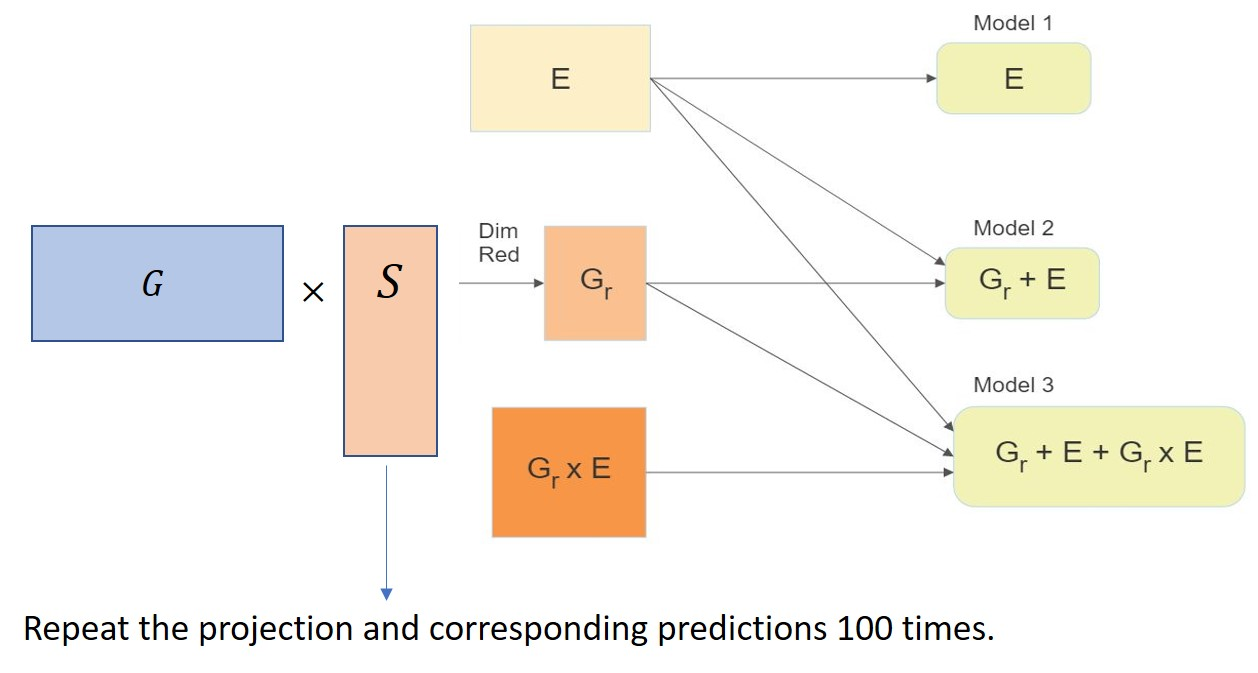
\includegraphics[scale=0.4]{figures/rp_2_1.jpg}
\caption{Implementation of the random projection algorithm for dimensionality reduction of the genomic data set in the genomic prediction problem.}
\label{fig:rp_implement}
\end{figure}
\end{center}

\subsection{Random Sampling}

Random sampling is another randomized approach to address the non-uniformity structure of data and form lower-dimension approximation matrices. While random projection addresses the non-uniformity by "uniformizing" the structure through rotations, random sampling algorithms build an importance probability to address the non-uniformity. We will describe the naive approach to random sampling followed by a simple random sampling algorithm. The naive random sampling algorithm does not apply any methods to bound the approximation error, but acts as an ideal introduction to these sampling algorithms. \\

The random sampling approach involves sampling a small number of features that represent the whole set of features. The naive approach randomly selects the features with uniform probability in independently and identically distributed (IID) trials. This approach ignores the non-uniformity structure presented in the data by giving an equal probability to each feature of the original predictor data. The reduced feature set could lose crucial information and structure from the original data. Hence, the naive uniform  sampling is not a popular choice of method for dimensionality reduction.\\

A more reasonable approach is to quantify the non-uniformity structure using some measure. Earlier, we had introduced statistical leverage scores. These leverage scores can be interpreted as a measure of influence the data points have on related computations and hence can be viewed as a metric to define the non-uniformity in the original matrix. Recall that the leverage score of the i-$th$ column of a matrix is given by $l_i = ||V'_(i)||_2^2$.
Since, $\sum_{i=1}^n l_i = ||V'||^2 = d$, we can define a probability distribution over the columns of $\textbf{A}$ given by $p_i = l_i/d$. We will refer to this probability distribution as the importance probability distribution which is a measure of the relative importance of columns in the matrix. It provides a probability distribution based on which the random sampling can be carried out while accounting for the non-uniformity structure of the original matrix. \\

As discussed earlier, the computational bottleneck for using importance probability distribution lies in its dependence on computation of the orthogonal basis for the input matrix. \cite{drineas_fast_2012} provided an algorithm to compute the relative-error approximate leverage scores $l_i$ instead of the computing the exact statistical leverage scores. Their contribution was a key development in the area of random sampling algorithms. We used their algorithm as the basis for implementing the random sampling algorithm in the genomic prediction problem. \\

We now describe the random sampling algorithm presented in \cite{drineas_fast_2012} along with drawing the attention of the reader to the salient properties and contributions. Consider a matrix $\textbf{A} \in \mathds{R}^{n \times d}$ with $d >> n$ and let $V'$ be the corresponding right singular matrix of $\textbf{A}$. Principally, we are interested in approximating the statistical leverage scores $l_i$ of the columns of $\textbf{A}$, which are then used to construct the importance probability distribution.

\begin{equation} \label{eq:2}
l_i = \left\Vert V'_{(i)}\right\Vert_2^2 = \left\Vert e'_i\ V' \right\Vert_2^2
\end{equation}

\noindent where $e_i$ is the $i$-th standard basis vector. The computation of the orthogonal matrix $V'$ takes $O(n^2d)$ time, which is the bottleneck. Since $V'$ can also be seen as any orthogonal basis for the column space of $\textbf{A}$, it follows that $V'V = AA^+$ where $^+$ is the Moore-Penrose inverse. From this, we can redefine the statistical leverage scores as,

\begin{equation} \label{eq:3}
l_i = \left\Vert e'_i\ V' \right\Vert_2^2 = \left\Vert e'_i\ V'V \right\Vert_2^2 = \left\Vert e'_i\ AA^+ \right\Vert_2^2.
\end{equation}

The computational complexity of calculating the leverage scores according to Eqn. \ref{eq:3} involves computing the pseudo-inverse $\textbf{A}^+$ and performing the matrix multiplication of $\textbf{A}$ and $\textbf{A}^+$. We apply random projection to overcome both these complexities by performing the computations and finally obtaining the approximate leverage scores $\tilde{l}_i$. \\ 

Instead of computing $\textbf{A}^+$, we find a smaller matrix that approximates $\textbf{A}$ and find the corresponding Moore-Pensore inverse of the smaller matrix. Subsampled Randomized Hadamard Transform (SRHT) is used to derive the smaller matrix as it preserves the structure $\textbf{A}$. SRHT rotates $\textbf{A}$ to a random basis where all the rows have an equal influence and uniformly samples rows from that basis. If $\Pi_1 \in \mathds{R}^{r_1 \times n}$ is a $\epsilon$-FJLT matrix for $V'$, then $\Pi_1 \textbf{A}$ is the approximation of $\textbf{A}$. Then Eqn. \ref{eq:3} becomes,

\begin{equation} \label{eq:4}
\hat{l}_i = \left\Vert e'_i\ A(\Pi_1 A)^+ \right\Vert_2^2.
\end{equation}

While computing the product $\textbf{A}\textbf{A}^+$ takes $O(nd^2)$, the computation of $\textbf{A}(\Pi_1 \textbf{A})^+$ takes $O(ndr_1)$ time. This is not efficient since $r_1 > d$. Since only the Euclidean norms of the rows of $\textbf{A}(\Pi_1 \textbf{A})^+$ are required, the dimensionality of this matrix can be reduced by using a $\epsilon$-JLT for the rows of $\textbf{A}(\Pi_1 \textbf{A})^+$. Suppose $\Pi_2 \in \mathds{R}^{r_1 \times r_2}$ is an $\epsilon$-JLT, then $\textbf{A}(\Pi_1 \textbf{A})^+ \Pi_2$ is a randomized sketching of $\textbf{A}\textbf{A}^+$. Then we can compute the approximate statistical leverage scores as

\begin{equation} \label{eq:5}
\tilde{l}_i = \left\Vert e'_i\ A(\Pi_1 A)^+\Pi_2 \right\Vert_2^2.
\end{equation}

 \cite{drineas_fast_2012} showed that for any error parameter $\epsilon \in (0, 0.5]$ and any arbitrary matrix $\textbf{A}$ of size $n \times d$ with $n >> d$, the expression 

\begin{equation}
|l_i - \tilde{l}_i| \leq \epsilon l_i 
\end{equation}
 holds for all $i = 1, 2, \dots, n$. \\

This result can be  extended without loss of generality for $d >> n$ case as well. \cite{ma_statistical_2015} investigated the approximation quality for several combinations of $r_1$ and $r_2$ through simulation studies. They found that $r_1$ does not have a significant impact on the correlation between approximate and exact leverage scores but running time increases linearly with $r_1$. On the other hand, the correlations between approximate and exact leverage scores increase rapidly with increasing $r_2$, but $r_2$ does not impact running time. Thus, they concluded that a combination of small $r_1$ and large $r_2$ would result in high-quality approximations with short run time. \\

\subsubsection{Implementation of the random sampling algorithm}

We used the statistical leverage scores to calculate the importance probability distribution required for the random sampling algorithm. We followed the two stage algorithm presented by \cite{boutsidis_improved_2009} to implement the random sampling algorithm. The implementation of the random sampling algorithm for dimensionality reduction of the marker data set for genomic prediction is as follows:


\begin{enumerate}
    \item Compute the approximate leverage scores as defined in \cite{drineas_fast_2012}.
    \item Use the approximate leverage scores to define the importance sampling distribution for the columns of the input marker matrix $X$.
    \item Randomly sample predefined number of columns $k$ according to the importance sampling distribution to form reduced matrices of different sizes.
    \item Use the reduced matrix $X$ to compute the genomic effect $G = XX'$ as the input for the prediction models and obtain predictions in all cross-validation schemes. 
    \item Repeat steps 3-4 100 times to remove sampling bias from the prediction accuracy results.  
\end{enumerate}

The advantage of this random sampling algorithm is the computation of the approximate leverage scores instead of the exact scores, effectively reducing computation time. In the next section, we describe another randomized algorithm for dimensionality reduction based on clustering. \\


\subsection{Clustering}
\label{sec:clustering}

Clustering is the process of grouping a set of objects in such a way that objects in the same group are more similar to each other than to objects in different groups, called clusters. Grouping objects when the data are labeled is a trivial task and is often referred to as supervised classification \cite{jain_data_1999}. But, often we are presented with data with no labeling available. Clustering was developed as a tool to deal with problems where the objective was to group unlabeled objects into meaningful collections. Because of the absence of labels, clustering is also called as unsupervised classification. \\

Clustering has seen immense interest in recent decades through its various applications in pattern and object recognition, recommender systems, and machine learning. It was first introduced in anthropology by Driver and Kroeber (1932) where they grouped cultures from different tribes of Polynesia and the Americas based on the presence or absence of traits such as matrilineage, sinew-backed bow, twined weaving, ridged houses, etc. Over the years clustering has been applied as a classification tool in many fields such as social science, psychology, biology, marketing, medicine, etc \cite{Hartigan1975, Punj1983, Jiang2004, Clatworthy2005, Sutherland2012}. Clustering is also used for detecting anomalies in the data, for identifying degree of similarity of objects, and for organizing and summarizing data. \\

The general scheme of clustering is to start with $n$ objects and sort them into $K$ groups based on some similarity measure such that the intra-group similarity is high and the inter-group similarity is low. Several categorizations of the clustering algorithms are available. Clustering algorithms can be broadly divided into partitional and hierarchical algorithms \cite{fraley_model-based_2002}. \cite{xu_comprehensive_2015} classified the clustering algorithms into traditional and modern each with 9 categories and 10 categories, respectively. Developing clustering algorithms is not the focus of this paper, so we will discuss only partitional and hierarchical clustering algorithms and use them as a means to compare clustering to the other dimensionality reduction algorithms. \\

\subsubsection{Partitional Clustering Algorithm}

Partitional clustering divides the set into non-overlapping subsets (clusters) such that each object is present only in one cluster. Typically, partitioning clusters produce clusters by optimizing some criterion function to produce optimal solutions \cite{Hartigan1975}. K-means, the most popular partitional algorithm, is an algorithm  where the objective is to minimize the sum of the squares of the distances from the objects to the centroid of the cluster. K-means algorithm ensures that there are always exactly $k$ clusters at the end of the process, with each cluster containing at least one item. \\

The general form of the k-means algorithm is as follows:

\begin{enumerate}
\item Choose the number of cluster, $k$.
\item Randomly assign $k$ out of $n$ items as cluster centroids.
\item Assign all the remaining $(n-k)$ items in the collection to their nearest cluster based on distance to the centroid.
\item Recompute the cluster centroids based on the current cluster assignment. 
\item Reassign items to their nearest cluster based on distance to centroids.  
\item Repeat steps 4-5 until no items change cluster assignments, or an iteration threshold is met. 
 \end{enumerate}

K-means clustering is a very efficient and easy algorithm to apply. However, it may not be a suitable algorithm in certain cases:

\begin{itemize}
\item \textbf{Non-globular cluster:} The solution to the k-means clustering is obtained by minimizing the within-cluster sum of squares. This is minimized when the clusters are globular and when the clusters are well separated from each other. Thus, applying k-means to non-globular shapes leads to results that are not optimal. Non-globular clusters can be visualized as in Figure \ref{fig:nonglob}.

\item \textbf{Non-uniform cluster sizes:} The cluster sizes are expected to be more or less similar to each other. K-means algorithm is not suitable when there is large variation in the cluster sizes from one cluster to the next. This issue is depicted in Figure \ref{fig:diffsizes}.

\item \textbf{Presence of outliers:} K-means algorithm is sensitive to outliers. The algorithm updates the centroids of the clusters by taking the average of all the points in the cluster. The presence of outliers will pull the centroid towards the outliers and lead to mis-classification of data points into the wrong clusters. There are several solutions in the literature to perform k-means in the presence of outliers \cite{dave_robust_1997, gan_k_2017, jiang_giniclust_2016, hautamaki_improving_2005}.

\begin{figure}[!htp]
  \centering
  \subfloat[Non-globular clusters]{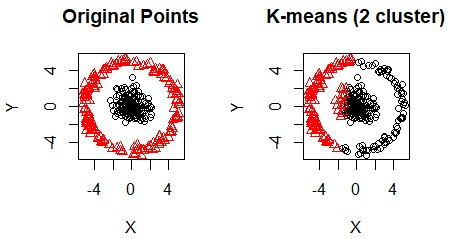
\includegraphics[width=0.5\textwidth]{figures/kmeans2_compiled.jpg}\label{fig:nonglob}}
  \hfill
  \subfloat[Non-uniform cluster sizes]{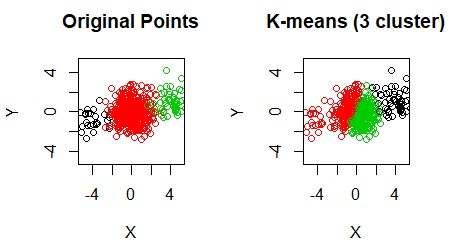
\includegraphics[width=0.5\textwidth]{figures/kmeans1_complied.jpg}\label{fig:diffsizes}}
  \caption{Limitations of K-means algorithm\\}
\end{figure}

\end{itemize}

Some of the drawbacks such as the need for globular clusters and the need for cluster sizes to be similar can be overcome by using a hierarchical clustering approach rather than a partitional clustering algorithm. We expand on the hierarchical clustering method in the next section. 

\subsubsection{Hierarchical Clustering Algorithm}

Hierarchical clustering is the process of creating a set of nested clusters arranged into a tree or dendrogram structure. Hierarchical clustering does not require a determination of the number of clusters $k$ prior to the clustering process, as opposed to the k-means clustering. The nested structure provides flexibility of choosing the number of clusters based on the dendrogram as well as domain expertise \cite{jain_data_1999}. There are two possible directions of clustering under hierarchical clustering: agglomerative (bottom-up) and divisive (top-down). In agglomerative clustering, each object is a cluster by itself initially and the most similar clusters are paired together successively to form a hierarchy. In divisive clustering, we start with the entire set of objects as one cluster and recursively divide each cluster into sub-clusters based on dissimilarity. Both these approaches lead to a hierarchy among objects which can be represented by a dendrogram. In this paper, we focus only on the agglomerative hierarchical clustering approach. A typical agglomerative hierarchical clustering scheme is given below:

\begin{enumerate}
\item Start with each item in its own cluster. 
\item Compute all similarity between all pairs of clusters. 
\item Merge the two clusters that are most similar to each other based on the clustering metric.
\item Repeat the process until only one cluster is remaining.
\end{enumerate}

The process of merging clusters at each iteration leads to a dendrogram depicting the hierarchy structure present. The merging of clusters is determined by clustering metrics which define the similarity among the clusters. There are several clustering metrics available in literature, some of which are presented in the next section. 

\subsubsection{Clustering Metrics}

There are several metrics that can be used to compute the similarity or dissimilarity between clusters. In this paper, we describe four of the most popular metrics: single-linkage \cite{sneath_numerical_1973}, complete-linkage \cite{king_step-wise_1967}, average-linkage \cite{eslr} and Ward's method \cite{murtagh_survey_1983, ward_hierarchical_1963}. \\

\textbf{Single-linkage}, also known as minimum linkage, method computes all pairwise distance between the elements within two clusters, and considers the smallest of these distances as a linkage criterion. The single-linkage algorithm is versatile in applications, but often tends to produce elongated clusters. To merge two clusters using single-linkage, only one object of the cluster needs to be close to the other cluster. Thus, this could lead to chaining and elongated clusters. Single-linkage also does not perform well if there is noise between clusters. In other words, single-linkage is not suitable if the clusters are not well separated. \\

\textbf{Complete-linkage} method considers the largest value (i.e., maximum value) of these distances as the distance between the two clusters. Complete-linkage method tends to produce more compact clusters and is also less susceptible to outliers and noise. It produces well-bounded compact clusters compared to single-linkage method, but tends to break large clusters into smaller ones. \cite{Jain1988} observed that complete-link is often the sensible option in most applications. \\

\textbf{Average-linkage} method computes all pairwise distances between elements in two clusters and takes the average of all distances as the distance between the two clusters. Average-linkage algorithm also performs well in the presence of noise between clusters. But like the complete-linkage algorithm, it tends to produce globular clusters. \\

\textbf{Ward's method}, or Ward's minimum variance method, computes the distance between two clusters as the increase in the total within-clusters sums of squares when two clusters are merged. The two clusters whose union leads to the smallest increase in the sum of the squares are merged together. Ward's method has the same disadvantages as complete-linkage, whereby it favors globular clusters. \\

Single-linkage is not the preferred metric due to its susceptibility to produce elongated clusters. Complete-linkage is avoided because of its inability to retain large clusters. Between average-linkage and Ward's minimum variance method, there is no real distinguishing factor. Since Ward's method can be compared easily to the objective function in k-means, we picked the Ward's method as our metric of choice for the hierarchical clustering approach.

\subsubsection{Implementation of clustering for dimensionality reduction}

In this section, we describe our approach to applying dimensionality reduction to genomic data sets with clustering acting as the reduction technique. Hierarchical clustering creates a nested clustering structure, often represented by a dendrogram. This allows the user to create any number of clusters by choosing the appropriate height to cut the dendrogram. One of our objectives was to study the trend in prediction accuracy as a function of the input data sizes. Thus, we are interested in creating reduced data sets of 26 different sizes. The K-means algorithm needs to be run 26 times to obtain the 26 different reduced marker data sets. On the other hand, hierarchical clustering needs to be performed only once to determine the hierarchy. The 26 different marker data sets can be created by cutting the dendrogram 26 times at appropriate heights. Thus, hierarchical clustering is computationally more efficient for our application and hence is the clustering algorithm of choice for this paper. \\

The R package $`fastcluster'$ \cite{mullner_fastcluster_2013} was used for fast implementation of the hierarchical clustering algorithm. The implmentation of the clustering algorithm for dimensionality reduction of the genomic data set can be summarized as follows:

\begin{enumerate}
    \item Perform agglomerative hierarchical clustering using $`fastcluster'$ to determine the hierarchy.
    \item Form $k$ clusters from the hierarchy by cutting appropriately.
    \item Sample one feature randomly from each of the $k$ clusters as the representative of that cluster.
    \item The sampled features form the reduced data set of size $k$ and will be used for the genomic prediction models.
    \item Repeat the sampling from the clusters and the following model implementation 100 times to remove sampling bias in the prediction accuracy results. 
\end{enumerate}

In the next sections, we describe two deterministic feature selection algorithms. First, we look at the deterministic sampling algorithm which is a deterministic analogue of the random sampling algorithm. 

\subsection{Deterministic Sampling}
\label{sec:det_sampling}

The feature selection method involves selecting a small subset of the original features to create the compressed feature matrix and hence avoids the issues with inference and  interpretability. Feature selection is also known as the column subset selection problem (CSSP) in matrix theory and linear algebra. Before we discuss the feature selection based dimensionality reduction approach in greater detail, we define CSSP formally.\\

\textbf{Column Subset Selection Problem: } Let $\boldsymbol{A} \in \boldsymbol{\mathds{R}}^{n \times d}$ and let $c < d$ be a positive integer. Select $c$ columns of A to form a matrix $\boldsymbol{C} \in \mathds{R}^{n \times c}$ that minimizes 

\begin{equation}
\left\Vert A - CC^+A \right\Vert_\xi 
\end{equation}

\noindent where $\textbf{C}^+$ denotes the Moore-Penrose inverse \cite{penrose_generalized_1955} of matrix $\textbf{C}$ and $\xi = \{2, F\}$, denotes the spectral or Frobenius norm \cite{meyer2000}, respectively. \\

Jolieffe \cite{jolliffe_discarding_1972} proposed one of the first column subset selection algorithms. The algorithm involved deterministic sampling of the columns of the matrix based on ordered leverage scores. While the algorithm led to favorable dimensionality reduction in many practical applications, they did not provide theoretical guarantees on the quality of the approximation and hence, it was not widely used. \cite{drineas_relative-error_2008} developed the randomized counterpart to the deterministic sampling algorithm that employs a sampling probability distribution based on the leverage scores. They proved that their algorithm produces a matrix $C$ that satisfies $\left\Vert A - CC^+A \right\Vert \leq (1+\epsilon) \left\Vert A - A_k \right\Vert $ with constant probability and hence guaranteed the approximation quality of their algorithm. Here, $A_k$ is the best rank-k approximation obtained from SVD and $c = O(k \log k / \epsilon^2)$ is the number of columns in $C$. \\

The randomized algorithm gives a `near-optimal' approximation of the matrix, but may not be computationally as efficient as the deterministic algorithm.  \cite{papailiopoulos_provable_2014} developed theoretical derivations for the approximation errors of the deterministic sampling algorithm provided by \cite{jolliffe_discarding_1972}. They proved that if the ordered leverage scores $l_i$  follow a steep enough power-law decay, then the deterministic algorithm performs equally or better than the randomized algorithm. Further, if the leverage scores follow a steep power-law decay, then the number of columns chosen by the deterministic algorithm is similar or fewer than the randomized counterpart as proposed by \cite{drineas_relative-error_2008}. They showed the utility of the power-law decay assumption by providing several examples of real data sets where the leverage scores followed a power-law decay. \cite{papailiopoulos_provable_2014} also emphasized that while their theoretical analysis was performed for the power-law decay model, other models for the leverage scores could be developed. \\

We now summarize the deterministic algorithm presented in \cite{papailiopoulos_provable_2014} as well as briefly state the theorems that guarantee the quality of the approximations produced from this algorithm. The proofs for the theorems are beyond the scope of this paper and detailed presentation of the proofs can be found in \cite{papailiopoulos_provable_2014}. \\

\noindent The deterministic algorithm can be described in 3 steps:

\begin{enumerate}
    \item Compute the top-$k$ right singular vectors $\textbf{V}_k$ of $\textbf{A}$ using SVD of $\textbf{A}$.
    \item Calculate the leverage scores $l_i^{(k)}$,  where the superscript refers to the choice of $k$ in the SVD. Reorder the leverage scores in a decreasing order. 
    \item Select $c$ columns of $\textbf{A}$ that correspond to the top $c$ leverage scores such that their sum is greater than some stopping threshold $\theta$, $\sum_{i=1}^c l_i^{(k)}>\theta$. The choice of $\theta$ controls the quality of the approximation. 
\end{enumerate}


\begin{algorithm}[t]
\SetAlgoLined
\KwIn{$\textbf{A} \in \mathds{R}^{n\times d}$, $k$, $\theta$}

1: Compute $A = U\Sigma V^T$, the singular value decomposition of $\textbf{A}$. Extract the top-$k$ right singular vectors of $\textbf{A}$, $\textbf{V}_k \in \mathds{R}^{d \times k}$.\\
2: \For{$i \gets 1$ \textbf{to} $d$} {
	$l_i^{(k)} = \left\Vert [V_k]_i, \right\Vert_2^2$
}
3 : Without loss of generality, let the leverage scores be sorted in decreasing order:
\begin{equation}
l_1^{(k)} \geq l_2^{(k)} \geq \cdots \geq l_d^{(k)}. \notag
\end{equation}
Sort the columns of $\textbf{A}$ according the leverage scores. Let the sorted column indices be $\pi_i$.\\ 
4: Find $c \in {1, 2, \cdots, n}$ such that 
\begin{equation}
c  = arg\min_c \left(\sum_{i = 1}^c l_i^{(k)} >\theta \right). \notag
\end{equation} 

5.  If $c<k$ from step 4, we set $c = k$. \\
6. Construct a subsampling matrix $\textbf{S} \in \mathds{R}^{d \times c}$. If the column $\pi_i$ is selected, then $S_{i,  \pi_i} = 1$ and 0 otherwise. \\
\KwOut{$\textbf{S} \in \mathds{R}^{d \times c}$ such that $C = AS$ contains top $c$ columns of $\textbf{A}$.}
 \caption{Deterministic Sampling Algorithm}
\end{algorithm}

The deterministic sampling algorithm requires the implementation of SVD to compute the leverage scores. Hence, the time complexity of the algorithm is given by $O(nd \min({n,d}))$. The resulting matrix from the deterministic sampling algorithm guarantees a bound on the approximation error with regard to the CSSP. This result is summarized in the following theorem whose proof can be found in \cite{papailiopoulos_provable_2014}. \\

\begin{theorem}[Deterministic Sampling]
Let $\theta = k - \epsilon$ for some $\epsilon \in (0,1)$. For a matrix $\textbf{C}$ obtained from the deterministic sampling algorithm and for $\xi = \{2,F\}$, we have
\begin{equation}
\label{eqn:thm1}
\left\Vert A - CC^+A \right\Vert_\xi^2 < (1-\epsilon)^{-1}\cdot \left\Vert A-A_k  \right\Vert_\xi^2. 
\end{equation}
\end{theorem}

In other words, the deterministic sampling theorem (DS theorem) shows that when a compressed matrix is derived using the deterministic sampling algorithm, the approximation error is at most $(1-\epsilon)^{-1}$ times the best approximation error obtained by the SVD method. DS theorem proves the existence of a high quality approximation matrix using the deterministic sampling algorithm and provides bounds for the possible values of $c$. More specifically, it dictates that the number of columns sampled is at least $k$, i.e., $c \geq k$. In the worse case scenario where the leverage scores follow a uniform distribution, the number of columns required to be sampled approaches $d$, where d is the total number of columns in the original matrix. \cite{papailiopoulos_provable_2014} further state that when the leverage scores exhibit a power-law decay, the number of columns selected by the deterministic sampling algorithm can be determined exactly. This is stated formally in the following theorem. 


\begin{theorem}[Power Law]
Let the leverage scores follow a power-law decay of the form:
\begin{equation}
\label{eqn:powerlaw}
l_i^{(k)} = \frac{l_1^{(k)}}{i^{\alpha_k}}
\end{equation}
where, $\alpha_k = 1+\eta$ for $\eta >0$. If we set the stopping threshold $\theta = k-\epsilon$ where $0<\epsilon<1$,  then the number of columns sampled by Algorithm 1 is:
\begin{equation}
c = \max \left\{\left( \frac{2k}{\epsilon} \right)^{\frac{1}{1+\eta}}-1, \ \ \left( \frac{2k}{\eta \cdot \epsilon} \right)^{\frac{1}{\eta}}-1,\ \  k \right\}.
\end{equation}

\end{theorem}

The corresponding subsampled matrix $\textbf{C}$ achieves the approximation error given in Eq. \ref{eqn:thm1}. \\

The deterministic sampling algorithm depends on two input parameters, $k$ and $\epsilon$. The parameter $k$ determines the rank of the SVD approximation of A, and the parameter $\epsilon$ determines the error tolerance when comparing $\textbf{C}$ to $\textbf{A}_k$ from SVD. The implementation of the deterministic algorithm for the purpose of genomic prediction can be seen as a pre-processing step. Given a large genomic information matrix, we use the deterministic algorithm to create a compressed matrix that represents the whole matrix well. \\

\subsubsection{Implementation of the deterministic sampling algorithm}

The deterministic sampling algorithm implementation mimics the random sampling implementation without the randomized sampling based on the leverage scores. The deterministic sampling algorithm can be summarized as follows:

\begin{enumerate}
    \item Compute the approximate leverage scores as defined in \cite{drineas_fast_2012}.
    \item Arrange the leverage scores in decreasing order. 
    \item Pick the top $k$ leverage scored columns to form the reduced matrices.
    \item Use these reduced matrices as the input for the genomic prediction models. 
\end{enumerate}


\subsection{Shrinkage Methods}
\label{sec:shrinkage methods}
Variable selection is the process of choosing a subset of the explanatory variables to explain a response variable. Variable selection helps in making models easier to interpret, reducing noise introduced by redundant variables, and reducing the size of the data set for faster computations. For these reasons, variable selection proves to be an important step in the analysis of high-dimensional data where the implementation and interpretation of models are made difficult due to the large number of variables present. \\


When the number of variables is very large, traditional subset selection methods have significant drawbacks. The best subset selection method involves fitting separate models for each possible combination of the $p$ predictors. For a problem with $p$ predictors, there are $2^p$ possible subset selections. The task of finding the "best" subset is practically unfeasible as $p$ increases. Stepwise selection methods are an alternative to the best-subset-selection method. They fit only a restricted set of models as opposed to the best-subset-selection method. Forward and backward stepwise selection are the two popular stepwise  selection algorithms. Both evaluate only $1+p(p+1)/2$ models compared to the $2^p$ models that are evaluated by best-subset-selection. Even though both these algorithms do not guarantee finding the "best" model containing a subset of the $p$ predictors, they are known to perform well in practice \cite{james_introduction_2013}. In high dimensional problems where $p > n$, backward selected cannot be used because of the initialization of the algorithm by fitting the full model. Forward selection can be used even when $ p > n$ as its initialization depends on fitting the null model containing no predictors. \\

Another drawback of the  traditional subset selection methods is the discrete nature of the variable selection, i.e., the variables are either retained or discarded. This leads to unstable variable selection, where a small change in data can lead to large change in the subset selected \cite{breiman_heuristics_1996}. Shrinkage methods were developed to address the shortcomings of the subset selection methods. These methods are also known as regularization or penalized methods. They work on the principle of imposing a constraint term that penalizes for model complexity. Shrinkage methods help in variable selection as well as improving the model's prediction performance through the bias-variance trade-off. In other words, shrinkage methods may provide solutions that have lower variance and higher bias, but ultimately leading to better prediction accuracy according to the mean squared error (MSE). \\

In this paper, we investigate the shrinkage methods as a tool for variable selection. We use the coefficients of the predictors, obtained from the shrinkage methods, as a form of ranking for variable selection. Our objective is to study how well the predictors are able to explain the response, as the number of predictors selected increases. In the following section, we describe the three popular shrinkage methods - LASSO, ridge regression, and elastic net  - along with their respective advantages and drawbacks. \\

\subsubsection{Ridge Regression}

Consider a standard linear regression model, 

\begin{equation}
y_i = \beta_0 + \sum_{j = 1}^p \beta_j X_{ij} + \epsilon \notag
\end{equation}

\noindent where $y_i$ is the response value for the $i$-th observation, $X_{ij}$ represents the $j$-th predictor for the $i$-th observation, and $\beta_j$ is the coefficient of the $j$-th predictor. The coefficients $\beta_j$ can be estimated as the values that minimize the residual sum of squares (RSS) function, 

\begin{equation}
RSS = \sum_{i = 1}^n \left( y_i - \beta_0 - \sum_{j = 1}^p \beta_j x_{ij} \right)^2.
\end{equation}

The estimates obtained by minimizing the RSS are known as the ordinary least squares (OLS) estimates. The OLS estimates are reliable only if the predictors are orthogonal. Further, if we have a high-dimensional problem with $p > n$, then OLS does not have a solution. Ridge regression was proposed by Hoerl and Kennard in 1970 as a solution to problems where OLS estimates are unreliable \cite{hoerl_ridge_1970}. While OLS estimates are unbiased, ridge regression estimates are biased. But, the increase in bias is compensated by a decrease in variance and results in estimates with smaller MSE. \\

Ridge regression is similar to least squares regression, but the estimates are obtained by minimizing a different objective function. In OLS, the coefficients are estimated by minimizing the RSS function. In ridge regression, the coefficients $\beta_j$ are estimated by minimizing a penalized residual sum of squares, 

\begin{equation}
\sum_{i = 1}^n \left( y_i - \beta_0 - \sum_{j = 1}^p \beta_j x_{ij} \right)^2 + \lambda \sum_{j = 1}^p \beta_j^2 = RSS +  \lambda \sum_{j = 1}^p \beta_j^2,
\end{equation}

\noindent where $\lambda\geq 0$ is a penalty parameter. $\lambda\sum_{j =1}^p \beta_j^2$ is called the penalty term and we note that it takes an $L_2$ penalty form. $\lambda$ controls the amount of shrinkage of the parameters $\beta_j$. The larger the penalty parameter, the greater the amount of shrinkage and the greater the coefficients are shrunk towards 0. When $\lambda=0$, the ridge regression estimates are equal to the OLS estimates. At $\lambda = 0$, the variance is high and the bias is low. As $\lambda$ increases, the variance reduces substantially but the bias increases only marginally. Thus, ridge regression provides equally or more accurate predictions compared to OLS regression. Further, if $p>n$, OLS does not provide unique solution whereas ridge regression can perform well by exploiting the bias-variance trade-off. \\

In ridge regression, the penalty parameter has to be estimated separately. There are several methods for estimating the most appropriate penalty parameter $\lambda$. The most popular and reliable method is cross-validation. We can choose a range of $\lambda$ values, compute the cross-validated error for each value of $\lambda$ and pick the $\lambda$ corresponding to the smallest cross-validation error \cite{james_introduction_2013}. Another method is to pick $\lambda$ by an automated procedure as proposed by \cite{hoerl_ridge_1975}. They proposed selecting the value of the penalty parameter as $\lambda = \frac{rs^2}{\sum_{j = 1}^p \hat{\beta}_j^2}$, where $r$ is the number of parameters in the model, $s^2$ is the RSS from the least squares estimation, and $\hat{\beta}_j$ are the least square estimates of the regression coefficients. \\
 
Ridge regression uses all the $p$ predictors in the final model. The term $\lambda\sum_{j = 1}^p \beta_j^2$ shrinks all coefficients towards 0, but does not set any of them exactly equal to zero. Hence, none of the predictors are removed from the final model. This can be perceived as a disadvantage in the context of the variable selection problem. In this paper, our focus is on reducing the dimensionality of the data using variable selection. Both subset-selection and dimension reduction methods lead to reducing the number of predictor variables used in the final model. Thus, another shrinkage method called Least Absolute Shrinkage and Selection Operator (LASSO) was proposed by  Tibshirani in 1996 \cite{tibshirani1996} that overcomes this disadvantage and allows the shrinkage to be 0. \\ 

\subsubsection{LASSO}

LASSO is a shrinkage method that applies an $L_1$ penalty on the regression coefficients. In ridge regression, an $L_2$ penalty was applied. Due to the nature of the $L_1$ penalty, LASSO performs both shrinkage and automatic variable selection \cite{tibshirani1996}. In other words, the penalty term not only shrinks the coefficients towards 0, it sets some of the coefficients to 0. Thus, LASSO inherently `eliminates' the predictors from the final model that have coefficients 0, . \\

In ridge regression, the coefficients are estimated by minimizing a penalized residual sum of squares with a $L_2$ penalty. With LASSO, the coefficients $\beta_j$ are estimated by minimizing a penalized residual sum of squares with an $L_1$ penalty:

\begin{equation}
\sum_{i = 1}^n \left( y_i - \beta_0 - \sum_{j = 1}^p \beta_j x_{ij} \right)^2 + \lambda \sum_{j = 1}^p | \beta_j | = RSS +  \lambda \sum_{j = 1}^p | \beta_j | ,
\end{equation}

\noindent where $\lambda \geq 0$. When the penalty parameter $\lambda$ is sufficiently large, some of the coefficient estimates are set to be exactly equal to 0. A detailed explanation of why LASSO sets some coefficients to 0 while ridge regression does not, can be found in \cite{tibshirani1996} and \cite{james_introduction_2013}. Thus, LASSO performs variable selection. As with the ridge regression, when $\lambda  = 0 $ the LASSO estimates are equivalent to the OLS estimates. The penalty parameter $\lambda$ has to be estimated separately, similar to ridge regression. The cross-validation method of searching for optimal value of $\lambda$ works with LASSO as well and is the most popular one. \\

LASSO has its own set of disadvantages. When $p>n$, LASSO selects at most $n$ variables \cite{zou_regularization_2005}. Further, LASSO selects only one variable at random from a group of high correlated variables. This can be a significant drawback in situations where selecting one of the variables from the group implies that all other variables are important as well because LASSO selects only one and discards the rest of the variables in the group. \cite{zou_regularization_2005} proposed a new shrinkage method called the elastic net to overcome the problems presented by LASSO while retaining the advantages of LASSO. \\


\subsubsection{Elastic Net}

Elastic net can be viewed as a combination method involving both ridge regression and LASSO \cite{zou_regularization_2005}. In elastic net, the coefficients $\beta_j$ are estimated by minimizing a penalized residual sum of squares with an elastic net penalty term:

\begin{eqnarray}
\sum_{i = 1}^n \left( y_i - \beta_0 - \sum_{j = 1}^p \beta_j x_{ij} \right)^2 &+& \lambda \sum_{j = 1}^p \left( (1-\alpha) |\beta_j| + \alpha \beta_j^2 \right) \notag \\
= RSS &+&  \lambda \sum_{j = 1}^p \left( (1-\alpha) |\beta_j| + \alpha \beta_j^2 \right) ,
\end{eqnarray}

\noindent where $\alpha = \frac{\lambda_2}{\lambda_1+\lambda_2}$. Here, $\lambda_1 \geq 0$ and $\lambda_2 \geq 0$ are penalty parameters. $\left( (1-\alpha) |\beta_j| + \alpha \beta_j^2 \right)$ is called the elastic net penalty term. When $\alpha=0$, elastic net is equivalent to the ridge regression and when $\alpha = 1$, elastic net is equivalent to LASSO. \\

Elastic net allows for variable selection and also allows for group selection of variables, acting as an ideal combination of ridge regression and LASSO. It is appropriate for scenarios where $p > n$. Similar to ridge regression and LASSO, appropriate values for the penalty parameters have to be estimated separately. The cross-validation method performs well for elastic net as well. It should be noted that instead of searching among a range of possible values for the penalty parameter, elastic net requires searching among a grid of values corresponding to the two penalty parameters present. \\

LASSO and elastic net perform variable selection along with model fitting. Unfortunately, they do not provide control on the number of variables selected or left out of the final model. To answer all the objectives of the study, we needed fine control on the number of variables selected by each reduction method. Ridge regression performs shrinkage on the coefficients associated with the variables, but does not perform variable selection of any kind. Thus, we picked ridge regression as the shrinkage method of choice. 

\subsubsection{Implementation of ridge regression for dimensionality reduction}

We used the $`glmnet'$ \cite{glmnet} package in \textbf{R} to implement ridge regression. Ridge regression is the only method of the five that takes the information from the response into the feature selection. Given below is the implementation of the ridge regression algorithm for dimensionality reduction of the genomic data set for genomic prediction:

\begin{enumerate}
    \item Implement a ridge regression model on the entire data set with the genotypic data.
    \item Use the coefficients estimated from the ridge regression as a measure of importance of the features. 
    \item Order the features by their respective regression coefficients.
    \item Pick the top $k$ features to form the reduced data set for the genomic prediction models. 
\end{enumerate}

\section{Data and Prediction Models}
\label{sec:gp and data}
\subsection{Data}

All of the methods were applied to a chickpea data set collected by the International Chickpea Screening Nursery (ICSN) of ICRISAT \cite{roorkiwal_genome-enabled_2016}.  The lines were phenotyped for three seasons (2012-13, 2013-14, and 2014-15) at two locations (ICRISAT, Patancheru and IARI, New Delhi) under different water regimes (normal-rainfed, irrigated and late-sown), which resulted in nine environments (season-by-location combinations). Phenotypic data on eight traits were collected: 100 Seed Weight (100-SDW), Biomass(BM), Days to 50\% Flowering (DF), Days to Maturity (DM), Harvest Index (HI), Plant Height (PH), Number of Plant Stand (PS) and Seed Yield (SY). In this paper, we focused on seed yield (SY) as the primary phenotype of interest. \\

The original data set contained 315 lines phenotyped in nine environments, giving a total of 2835 phenotypic yield observations. All of the 315 lines had corresponding genomic data with 26,817 markers each. The following steps were taken in the data-cleaning process:

\begin{enumerate}
    \item Removed all lines (rows in the data set) that had more than 90\% missing information in their genotypic data. This led to the deletion of 9 lines, leaving 306 lines in the data set.
    \item Removed the corresponding lines in the phenotypic data across all environments. 
    \item Removed all markers (features) with the Minor Allele Frequency (MAF) less than $0.05$. There were no features removed in this step. \item Removed all markers with more than 50\% missing values, leaving 14928 markers in the genotypic data set. 
    \item Imputed the remaining missing values in the marker data by taking the average of the rest of the entries in their respective columns. 
    \item Centered and scaled the genotypic data matrix.  
\end{enumerate}

After the cleaning process, the genomic data had 306 observations and 14,928 features, which could be viewed as matrix of size $306 \times 14928$. In the following section, we describe the models used for genomic prediction as well as the techniques used to evaluate the accuracy of the models. 

\subsection{Prediction Models}

In this paper, we used the models proposed by \cite{jarquin_reaction_2014} to evaluate  the predictive ability of reduced datasets. Specifically, we considered three models based on the input information in each model: either environmental and line information (E + L) only, or genomic information along with environment information (G + E), or genomic information with environmental information as well as their interactions (G $\times$ E) as the predictors. \\

Let the phenotypic trait be represented by $y_{ijk}$ for the $k$-th replicate for the $j$-th genotype or line in the $i$-th environment. Let the environmental effect be represented by $E_i \ (i = 1, 2, ..., I)$, the line effect be defined by $L_j \ (j = 1, 2, ..., J)$, the genetic effect be denoted by $g_j (j = 1, 2, ..., J)$, the interaction be denoted by $gE_{ij}$ and the error term be represented as $\epsilon_{ijk} \ (k = 1, 2, ..., r_{ij})$. The three models corresponding to the three scenarios mentioned above are given by:

\begin{eqnarray}
y_{ijk} &=& \mu + E_i + L_j+ \epsilon_{ijk}, \label{eq:e} \\
y_{ijk} &=& \mu + E_i + g_j + \epsilon_{ijk},\label{eq:g_e}\\
y_{ijk} &=& \mu + E_i + g_j + gE_{ij} + \epsilon_{ijk} \label{eq:gxe},
\end{eqnarray}

\noindent where $\mu$ is the overall mean, $E_i \sim N(0, \sigma_E^2)$, $L_j \sim N(0, \sigma_L^2)$, $\textbf{g} \sim N(\textbf{0}, \textbf{G}\sigma_g^2)$, $\textbf{gE} \sim N\left(\textbf{0}, [\textbf{Z}_g\textbf{G}\textbf{Z}'_{g}]\circ [\textbf{Z}_e\textbf{Z}'_e]\sigma_{gE}^2 \right)$ and $\epsilon_{ijk} \sim N(0,  \sigma_\epsilon^2)$; $\sigma^2_E, \sigma^2_g$, and $\sigma^2_\epsilon$ are environment, genetic and residual variances, respectively. $\sigma^2_{gE}$ is the variance component of the $\textbf{gE}$ interaction. $\textbf{Z}_g$ and $\textbf{Z}_e$ are incidence matrices for the effect of the genomic values and environment, respectively. $\textbf{G}$ refers to the genomic main effect, computed as $\textbf{G} = XX'/p$ where $X$ is the centered and scaled molecular markers matrix. Finally, $\circ$ denotes the Schur product (element by element product) between two matrices.\\

Through the dimensionality reduction methods, we reduce the size of the marker matrix (X) and thus the dimensionality reduction methods affect only the G + E (Eq. \ref{eq:g_e}) and G $\times$ E (Eq. \ref{eq:gxe}) models but not the baseline E + L model (Eq. \ref{eq:e}). \\

\subsection{Model assessment using cross-validation schemes}

Three different cross-validation schemes \cite{roorkiwal_genomic-enabled_2018} were implemented to assess the predictive ability of the models in different scenarios. These are scenarios that breeders might be interested in, since these mimic the situations they face in their breeding programs. The performance of the prediction models was assessed by measuring the Pearson correlations between the observed phenotypic values and the predicted genomic estimated breeding values within environments. The three different cross-validations are described below as, 

\begin{itemize}
\item \textbf{CV0} - prediction of lines in a new unobserved environment.
\item \textbf{CV1} - prediction of new untested lines in environments.
\item \textbf{CV2} - prediction of lines that were observed in some environments but not observed in other environments.
\end{itemize}

\textbf{CV0} refers to the cross-validation that evaluates the ability of the models to predict the performance of lines in a new unobserved environment. In effect, we performed a 9-fold cross-validation in which we leave out the observations from the observed target environment in each fold and use the other observations from the other eight as the training set. We computed the correlations between the observed and predicted values within each environment to determine the ability of the model to predict the performance of all the lines in a new environment. \\

\textbf{CV1} refers to the cross-validation that evaluates the ability of the models to predict the performance of untested lines in all environments. For CV1 a five-fold cross-validation scheme was used where we randomly selected 20\% of the lines as the testing group and left out all the observations corresponding to these lines from all environments. We used the observations from the other 80\% of the lines as the training set to build the prediction models. Then, we predicted the trait values for the lines that were left out across all environments. This process of creating folds randomly and performing predictions was repeated 20 times. Finally, we computed the correlations between the observed and predicted values within each environment and averaged them across the 20 runs to obtain the average correlations. \\

\textbf{CV2} refers to the cross-validation that evaluates the ability of the models to predict the performance of lines that were tested in some environments but not tested in other environments. For CV2, the phenotypic observations were randomly partitioned into five subsets without regard for the lines or environment. Four subsets were combined and used for training the models and the remaining subset was used as a test set. The process was repeated 20 times just as described in CV1 to obtain average correlations.  \\


\subsection{Dimensionality reduction in genomic prediction}

We investigated five dimensionality reduction methods in this paper. For each method, we performed feature selection/feature extraction to create reduced dimensional marker data sets of 26 sizes based on the number of markers present. The number of markers ranged from 200 to 14,928, which were all the markers available. We set the number of markers as fixed across all methods to be able to compare the dimensionality reduction methods and their prediction ability at each size. For the three randomized dimensionality reduction methods, 100 data sets were generated at each size and prediction results from the 100 data sets were averaged and set as the prediction accuracy of that size. This was done in order to overcome any bias that may have been introduced by the randomization process. For each reduced data set, we implemented the three predictions models (Eqs. \ref{eq:e}, \ref{eq:g_e}, \ref{eq:gxe}) and evaluated each model using the three cross-validation schemes described in the previous section. CV1 and CV2 cross-validation schemes were run 20 times on each set due to the randomization in the fold creation. Taking into consideration all the different methods, sizes, randomization, prediction models and cross-validation schemes, over 965,000 combinations were run in this study. 

\begin{figure}[H]
\centering
    \begin{subfigure}
       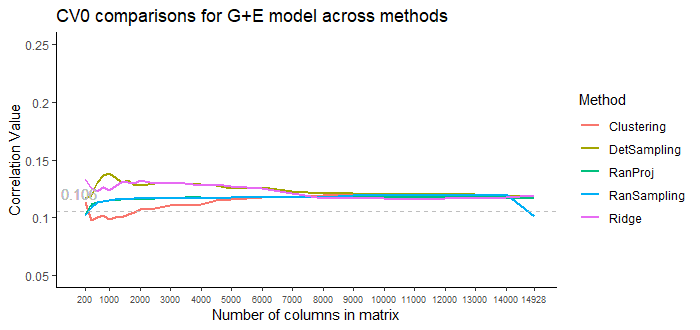
\includegraphics[width=0.9\linewidth]{figures/G+E_CV0_All_Methods.png}
       \label{fig:Ng1} 
    \end{subfigure}
    
    \begin{subfigure}
       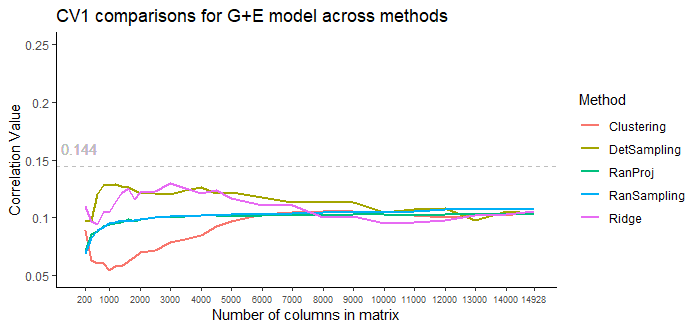
\includegraphics[width=0.9\linewidth]{figures/G+E_CV1_All_Methods.png}
       \label{fig:Ng2}
    \end{subfigure}
    
    \begin{subfigure}
       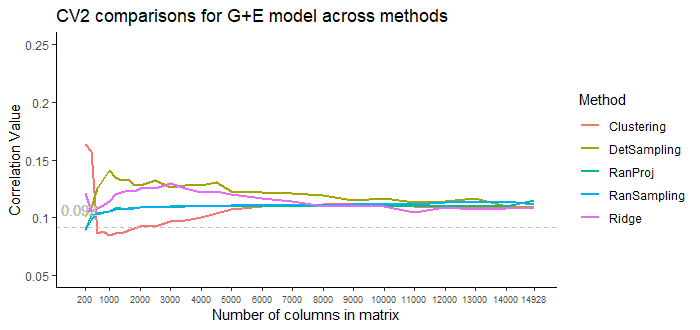
\includegraphics[width=0.9\linewidth]{figures/G+E_CV2_All_Methods.png}
       \label{fig:Ng3}
    \end{subfigure}
\caption{Prediction accuracy of a chickpea population comprising of 306 genotypes tested in 9 environments for the G+E model under the three cross-validation schemes (CV0, CV1, CV2) across 26 different genomic information sizes. \\}
 \label{fig:g_e_all}
\end{figure}

\begin{figure}[H]
\centering
\begin{subfigure}
   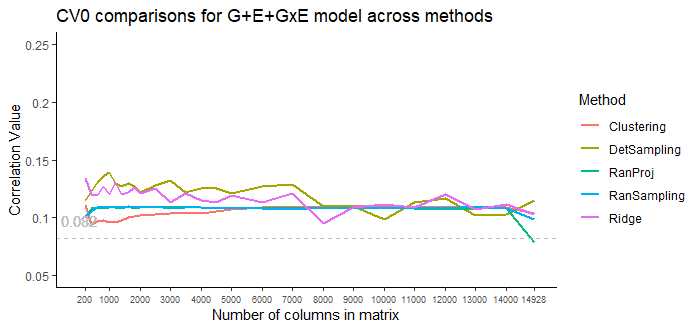
\includegraphics[width=0.9\linewidth]{figures/G+E+GxE_CV0_All_Methods.png}
   \label{fig:Ng4} 
\end{subfigure}

\begin{subfigure}
   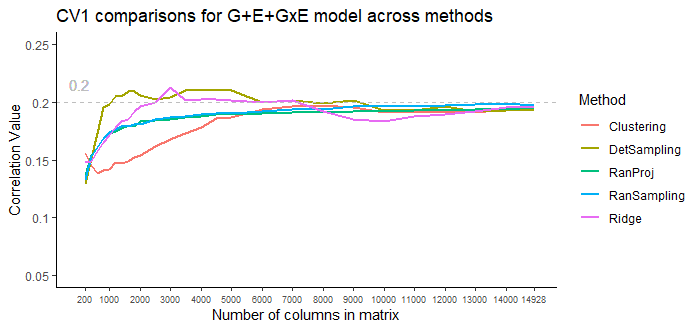
\includegraphics[width=0.9\linewidth]{figures/G+E+GxE_CV1_All_Methods.png}
   \label{fig:Ng5}
\end{subfigure}


\begin{subfigure}
   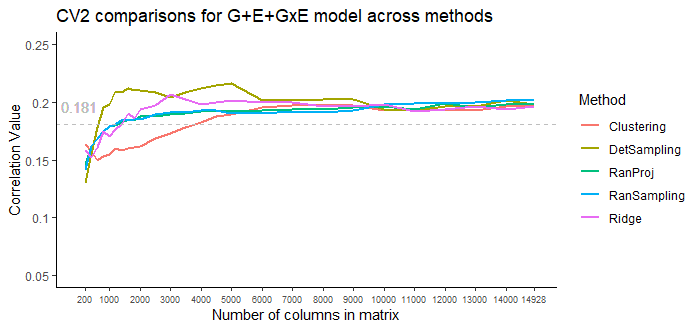
\includegraphics[width=0.9\linewidth]{figures/G+E+GxE_CV2_All_Methods.png}
   \label{fig:Ng6}
\end{subfigure}
\caption{Prediction accuracy of a chickpea population comprising of 306 genotypes tested in 9 environments for the G+E+GxE model under the three cross-validation schemes (CV0, CV1, CV2) across 26 different genomic information sizes. \\}
 \label{fig:gxe_all}
\end{figure}

\section{Results and Discussion}
\label{sec:results}

This study focused on two objectives. The primary objective was to evaluate the merit of using dimensionality reduction methods as a pre-processing step in genomic prediction. We used five dimensionality reduction methods in order to present dimensionality reduction as an effective pre-processing step in genomic prediction and compared their reduction capabilities to find which methods work better for genomic prediction. Second, we studied the trends in prediction accuracy of reduced data sets as a function of their size. \\

To recall, we compared the five dimensionality reduction methods using three genomic prediction models with each model evaluated using three cross-validation schemes. Among the prediction models, the model represented by Eq. \ref{eq:e} is a baseline model with only environmental and line effects. This model does not have genomic effects and hence are not subjected to any dimensionality reduction methods. Thus, the baseline $E+L$ model provides a single prediction accuracy value for each cross-validation scheme. For the other prediction models, each dimensionality reduction method was used to generate reduced marker data sets of 26 different sizes to answer our secondary objective. The results from these models are summarized in the plots in Fig \ref{fig:g_e_all} and Fig \ref{fig:gxe_all}. This chickpea data set was used for genomic prediction in \cite{roorkiwal_genomic-enabled_2018} using the same three genomic prediction models and evaluated with the same three cross-validation schemes. We used their prediction accuracy values as the benchmark to compare our results to. Their paper used the whole genomic data set without any dimensionality reduction and thus served well as a baseline to evaluate dimensionality reduction methods. For each model and cross-validation combination, their results are referenced using a grey horizontal line in the results. The differences in their results and our whole data set results are a consequence of the randomization in the cross-validation folds and hence are not a concern.\\

Irrespective of the model and CV scheme, all dimensionality reduction methods required only a fraction of the total input markers to obtain maximum correlation. In addition, we observed a plateauing of correlation values as the number of markers selected increased for all methods. Thus, the  number of markers required to achieve maximum correlation may be an inappropriate measure to evaluate the reduction capability of the method. Instead, we considered a 95\% of the maximum correlation as our metric to evaluate the reduction methods. For instance, for the CV1 scheme in the G $\times$ E model, the random projection algorithm achieved the maximum correlation of 0.195 with all 14,928 input markers. However, the method achieved a 95\% maximum correlation of 0.185 with just 3000 input markers. This is a significant reduction in the number of input markers for similar correlation values. In fact, for all the dimensionality reduction methods, fewer than 40\% of the input markers were required to achieve a 95\% max correlation value. These results are summarized in Table \ref{tab:cor_max}. Further, for the deterministic sampling and ridge regression based reduction, best correlation was achieved by a reduced data set rather than using the whole data set in all three models indicating the presence of noise in the data. This showed the usefulness of using dimensionality reduction methods as a pre-processing step in genomic prediction to reduce the noise in the data while maintaining or even improving the accuracy of the models. \\

Second, no one reduction method had the best reduction capability across all prediction models and CV combinations. For instance, for the CV2 scheme of the G $\times$ E model, deterministic sampling required only 1200 markers in the input data to achieve 95\% of the maximum correlation compared to 4500 required by clustering. On the other hand, for the CV2 scheme of the G + E model, clustering required only 200 input markers to attain 95\% of the maximum correlation compared to 1000 required by deterministic sampling. Random projection and random sampling methods were very similar to each other in terms of prediction accuracy values across all matrix size by model by cross validation combinations. All of the reduction methods had similar prediction accuracies within the model and CV combination, which reiterates the utility of dimensionality reduction regardless of the method used.



% Please add the following required packages to your document preamble:
% \usepackage{booktabs}
\begin{center}
\begin{table}[]
\centering
\begin{tabular}{@{}lllrr@{}}
\toprule
Pred. model & CV  & DR Method     & \# Cols & Correlation \\ \midrule
G+E+GxE    & CV0 & Clustering  & 200     & 0.105       \\
           &     & DetSampling & 800    & 0.132       \\
           &     & RanProj     & 400    & 0.104        \\
           &     & RanSampling & 400     & 0.104        \\
           &     & Ridge       & 200     & 0.127       \\
           \cline{2-5}
           & CV1 & Clustering  & 4500    & 0.185       \\
           &     & DetSampling & 1200    & 0.199        \\      
           &     & RanProj     & 3000   & 0.185       \\
           &     & RanSampling & 4000   & 0.189       \\       
           &     & Ridge       & 3000    & 0.202       \\ \cline{2-5}
           & CV2 & Clustering  & 4500    & 0.188       \\
           &     & DetSampling & 1200    & 0.205       \\       
           &     & RanProj     & 3000   & 0.189       \\
           &     & RanSampling & 3000   & 0.191       \\
           &     & Ridge       & 2500    & 0.197       \\ \cline{1-5}
G+E        & CV0 & Clustering  & 200    & 0.113       \\
           &     & DetSampling & 600    & 0.131       \\
           &     & RanProj     & 400    & 0.112       \\
           &     & RanSampling & 800   & 0.114        \\
           &     & Ridge       & 200     & 0.126       \\ \cline{2-5}
           & CV1 & Clustering  & 6000    & 0.101       \\
           &     & DetSampling & 800    & 0.123       \\
           &     & RanProj     & 1600    & 0.098       \\
           &     & RanSampling & 5000   & 0.103       \\
           &     & Ridge       & 1600    & 0.124       \\ \cline{2-5}
           & CV2 & Clustering  & 200     & 0.155       \\
           &     & DetSampling & 1000    & 0.134       \\
           &     & RanProj     & 2000   & 0.109       \\
           &     & RanSampling & 1800   & 0.108       \\
           &     & Ridge       & 1600    & 0.124       \\ \cline{1-5}
E+L        & CV0 &             & 14928   & 0.089       \\
           & CV1 &             & 14928   & -0.098      \\
           & CV2 &             & 14928   & 0.045       \\ \bottomrule
\end{tabular}
\caption{Number of markers selected by each dimensionality reduction (DR) method to obtain 95\% of the highest correlation for the three prediction models (G+E+GxE, G+E, E+L) under the three cross-validation schemes (CV0, CV1, CV2).}
\label{tab:cor_max}
\end{table}
\end{center}


\section{Conclusions}
\label{sec:conclusions}

Modern plant breeding programs rely on coupling genomic information with phenotypic performance data to select favorable lines. Early genomic selection models included line, environment, phenotypic and genomic information to predict the performance of lines. Complex traits such as yield are affected by a large number of genomic, environmental factors and their interaction and hence the development of models that allowed for this genotype by environment interactions improved the genomic prediction accuracy. The improvements in genotyping technology combined with the reducing cost has led to the generation of genomic data of enormous sizes which are often high-dimensional in nature. While current genomic selection models are capable of handling these high-dimensional data, there are questions about their efficiency. Further, including information on hundreds of thousands of potentially unrelated markers in the genomic prediction models could negatively impact the prediction accuracy of the trait of interest. Lastly, there is a computational resource cost that must be taken into account. Prediction models with larger input sizes require much greater computational resources to run, both in terms of hardware as well as time. We proposed dimensionality reduction as a mechanism to address all of these concerns.\\

In this study, we used a chickpea data set. Chickpea is the second largest produced food legume crop in the world \cite{roorkiwal_genome-enabled_2016}. It's high protein content makes it a valuable source of protein in several cultures across the world, especially in vegetarian diets. Implementation of GS methods helps breeding programs reduce breeding cycle time and improve the rate of genetic gains \cite{roorkiwal_genomic-enabled_2018} by allowing breeders to select lines using genomic marker data before performing field trials. With the recent improvements in the high-throughput genotyping technologies, millions of markers are available for several hundred lines of chickpea. GS has been adept at accessing these large data sets to predict performance of lines. However, further advances in this area will yield larger marker data sets which could potentially overwhelm the current GS methods as well as the computational resources available. In addition, other high-dimensional data such as high-dimensional weather covariates and high-throughput phenotyping information are increasingly more available in breeding programs. While we did not consider such data in this study, the inclusion of such data could create computational bottlenecks. These reasons present a need for developing methods that effectively handle large data sets and use the additional data available to improve prediction accuracies.  \\

The key contribution of this work was to propose using dimensionality reduction in genomic prediction analyses and show its utility using a handpicked subset of all available methods. For example, we explored the possibility of using randomized algorithms for dimensionality reduction with the help of primitive implementations. There are several more sophisticated randomized algorithms that could improve the dimensionality reduction, which can be explored in future works. Our results act as a proof of concept that future researchers can use to explore various dimensionality reduction methods and identify the best method for their breeding data. Our results clearly indicate the need for integrating dimensionality reduction methods into genomic selection to reduce the computational resource requirements and to improve the prediction process and better select the best performing lines in any breeding program. \\


\section{Acknowledgement}

This research was done using resources provided by the Open Science Grid \cite{osg07, osg09}, which is supported by the National Science Foundation award \#2030508. This work was completed utilizing the Holland Computing Center of the University of Nebraska,
which receives support from the Nebraska Research Initiative. VM was partially supported by the Development of Waxy Sorghum Lines Grant from the Department of Agriculture - NIFA (UNR 19-58). DJ was supported by the Agriculture and Food Research Initiative Grant (NEB-21-176) from the USDA National Institute of Food and Agriculture, Plant Health and Production and Plant Products: Plant Breeding for Agricultural Production, A1211, Accession No. 1015252.